\section{Applications}\label{sec:applications}

Both applications use the public interface of the software with $\alpha=0.05$, betting sequences with endpoint refinement, $n_0=b=5$, the optional cover phase described below, and a budget of $10^5$ evaluations. In both the true means can be computed exactly, so that each statement can be checked.

\subsection{Interval estimators for a binomial proportion}\label{sec:app-binomial}

Simulation studies of interval estimators report average coverage and length from a fixed number of replications \citep{morris2019}. We compare eight 95\% intervals for a binomial proportion with $n=30$: Wald, Wilson, Wilson with continuity correction (Wilson-cc), Agresti--Coull, Clopper--Pearson, Jeffreys, arcsine and likelihood ratio \citep{clopper1934,newcombe1998,agresti1998,brown2001}. The two objectives are the miscoverage and the width, averaged over $p\sim U(0,1)$. Both are bounded by $[0,1]$ and the truth is exact: given $X=x$, $p$ has a Beta$(x+1,n-x+1)$ distribution and $\Prob(X=x)=1/(n+1)$, so each method's average coverage is a finite sum of incomplete beta functions. Seven of the eight methods are Pareto-optimal; Wilson-cc is dominated by Clopper--Pearson by $0.0004$ in miscoverage and $0.0008$ in width (Table~\ref{S-tab:binomial} in the Supplementary Material). One evaluation is the average, over 100 simulated studies, of the miscoverage indicator and the width, and the tolerance is $0.005$ in both objectives, half a percentage point of coverage and $0.005$ in width.

All eight methods were accepted after 20{,}130 evaluations, that is, about $2\times10^6$ simulated studies (Figure~\ref{fig:applications}a). Five were certified optimal and three, Wilson-cc, Clopper--Pearson and likelihood ratio, were accepted as $\epsb$-Pareto-optimal; none was discarded, which is correct, because the only dominated method is dominated by much less than the tolerance. Deciding a difference of $0.0004$ in miscoverage would require intervals far narrower than any practical question needs. Since every method was accepted, the accepted set says little; the representatives say more. At acceptance they coincided with the plausible set, because the boxes were too wide to certify any cover. In the cover phase, which evaluates pairs of plausible alternatives until it is certified whether one $\epsb$-covers the other, they fell to four methods: Wald, Wilson, Agresti--Coull and Wilson-cc. Every Pareto-optimal method is therefore within $0.005$ in both objectives of one of these four, with probability at least $0.95$. The cover phase did not finish within the budget: eight ordered pairs remained undecided, and in each of them the true cover margin, the amount by which one method fails to be within $\epsb$ of the other or succeeds, is below $0.002$. This is the case that Theorem~\ref{thm:termination} does not reach. The usual table of estimated coverages and widths suggests a summary of this kind; the cover certifies it.

\subsection{Reorder policies for an inventory system}\label{sec:app-inventory}

The second application is a periodic-review $(s,S)$ inventory system with backlogging, modelled after the example of \citet[Section~1.5]{law2015}. Demand in each period is Binomial$(50,1/2)$; at the end of a period with inventory level $I<s$ an order of $S-I$ units is placed and arrives at the start of the next period. Each period costs 32 per order plus 3 per unit ordered, 1 per unit held and 5 per unit short. One evaluation is a replication of 60 periods after a warm-up of 20, and the two objectives are the average cost per period and the fraction of periods that end with a backlog. The $K=16$ policies cross $s\in\{10,20,30,40\}$ with $S-s\in\{20,40,60,80\}$. Because demand is bounded, the cost lies in $[0,832]$, a range about six times wider than the costs observed, and the backlog fraction in $[0,1]$; the two are correlated within a replication (about $0.5$). The level at the start of a period is a Markov chain on $\{s,\dots,S\}$, so both objectives are finite sums that we compute exactly; four policies are Pareto-optimal, all with $S-s=40$ (Table~\ref{S-tab:inventory}). The tolerance is one unit of cost and half a percentage point of backlog.

Every plausible policy was accepted after 59{,}510 evaluations (Figure~\ref{fig:applications}b). Seven policies were discarded, each with a plausible dominator named in the report; three were certified optimal; and six were accepted as $\epsb$-Pareto-optimal. Five of these six are dominated, among them $(40,100)$, which costs $3.8$ more per period than $(40,80)$ and, like it, runs out of stock in fewer than one period in $10^7$. We had not anticipated this when we chose the tolerance, but it follows from the definition: an alternative is $\epsb$-Pareto-optimal unless another improves on it by at least $\epsb$ in \emph{every} objective, and no policy can improve by $0.005$ on a backlog fraction below $0.005$. An alternative within $\varepsilon_i$ of the lower bound of objective $i$ is therefore never excluded by the target~\eqref{eq:target}, however large its disadvantage in the others. The representatives correct this: after the cover phase they are the three policies $(10,50)$, $(20,60)$ and $(30,70)$, which $\epsb$-cover the four Pareto-optimal policies; $(40,80)$ is represented by $(30,70)$, which costs $10$ less per period and runs out of stock in $0.05\%$ of periods. Here too the budget ended in the cover phase, with two pairs among the policies with $s\ge30$ undecided; neither involves a representative. The loose bound on cost was not costly because the betting sequences adapt to the small variance of the cost.

\begin{figure}[t]
\spacingset{1}
\centering
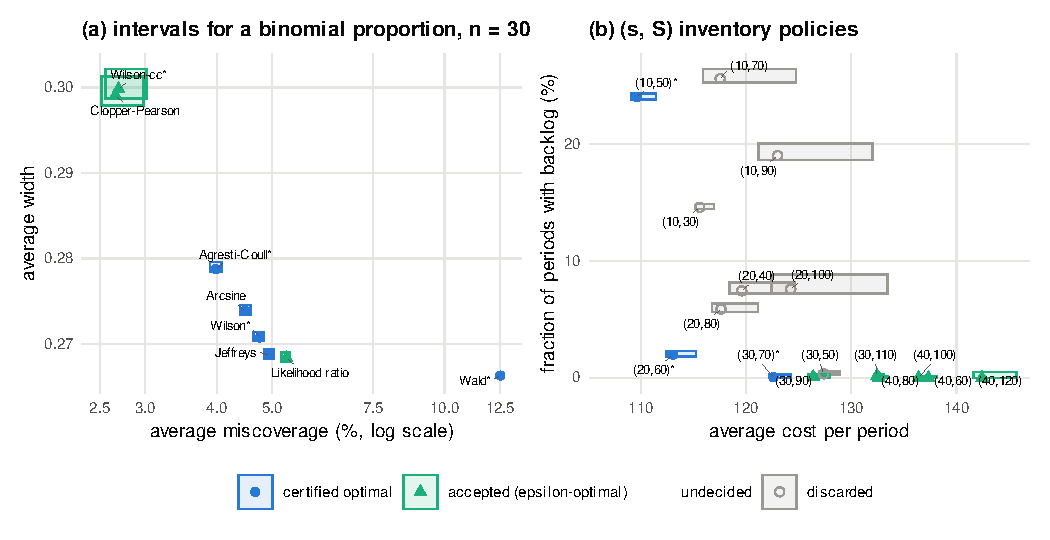
\includegraphics[width=\textwidth]{figures/fig3_applications.pdf}
\caption{The two applications at the end of one identification. Rectangles are the simultaneous confidence boxes, points are the true mean vectors, colour and shape give the status, and an asterisk marks the representatives. (a) Eight intervals for a binomial proportion with $n=30$; miscoverage on a logarithmic scale. (b) Sixteen $(s,S)$ inventory policies; the horizontal axis is restricted to the range of the boxes of the plausible policies.}
\label{fig:applications}
\end{figure}

To check the statements against the truth, each identification was repeated %APPREP% times with independent random numbers. %APPREPRESULT%
